% 2.3.CmakeLibrary.tex
%	Last update: 2019/07/24 F.Kanehori
%newpage
\subsection{dk1fTMPIllv1rQIl}
\label{subsec:CmakeLibrary}

\noindent
\KLUDGE 以下では、\cmake \KLUDGE の生成物(\KLUDGE ビルドの生成物ではありません)\KLUDGE を格納する
\KLUDGE 作業場所(\KLUDGE ディレクトリ)\KLUDGE を``\build''\KLUDGE として話を進めます(\KLUDGE 作業場所は任意で構いません)\KLUDGE 。

\medskip
\noindent
\cmake \KLUDGE にはConfigure\KLUDGE とGenerate\KLUDGE の2\KLUDGE 段階があります。

\medskip
\noindent
\KLUDGE コマンドプロンプトの場合は、1\KLUDGE 回のコマンドで両方を実行できます。
\Vskip{-.5\baselineskip}
\ifLwarp
	\begin{figure}[h]
	    \begin{center}
	    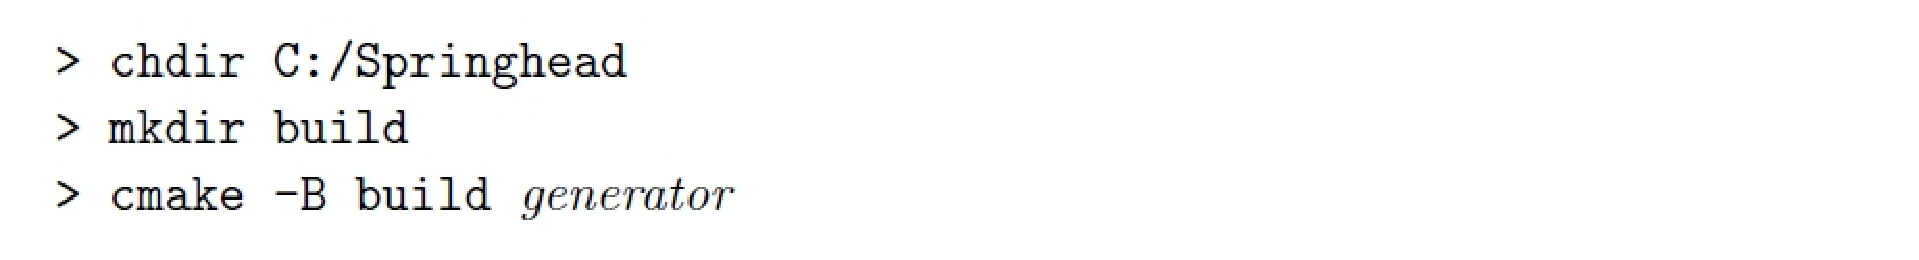
\includegraphics[width=\textwidth]{fig/command-2-3.eps}
	    \end{center}
	    \label{fig:DownloadTree}
	\end{figure}
\else
\begin{narrow}[15pt]
	\CmndBox{%
		\textgreater  chdir C:/Springhead\\
		\textgreater  mkdir build\\
		\textgreater  cmake -B build \it{generator}
	}
	\it{generator\KLUDGE の}\KLUDGE 詳細(\KQuote{\tt{-G "Visual Studio 15 2017" -A x64}}\KLUDGE など)\KLUDGE は、
	\KLUDGE コマンドプロンプトで\tt{cmake --help}\KLUDGE とすると確認できます。
\end{narrow}
\fi

\medskip
\noindent
GUI\KLUDGE の場合は、
\begin{narrow}[15pt]
	\KLUDGE まずConfigure\KLUDGE ボタン(\KLUDGE 図\ref{fig:CmakeConfigure} \KLUDGE 左図の下)\KLUDGE を押します。
	\begin{figure}[h]
	\begin{center}
	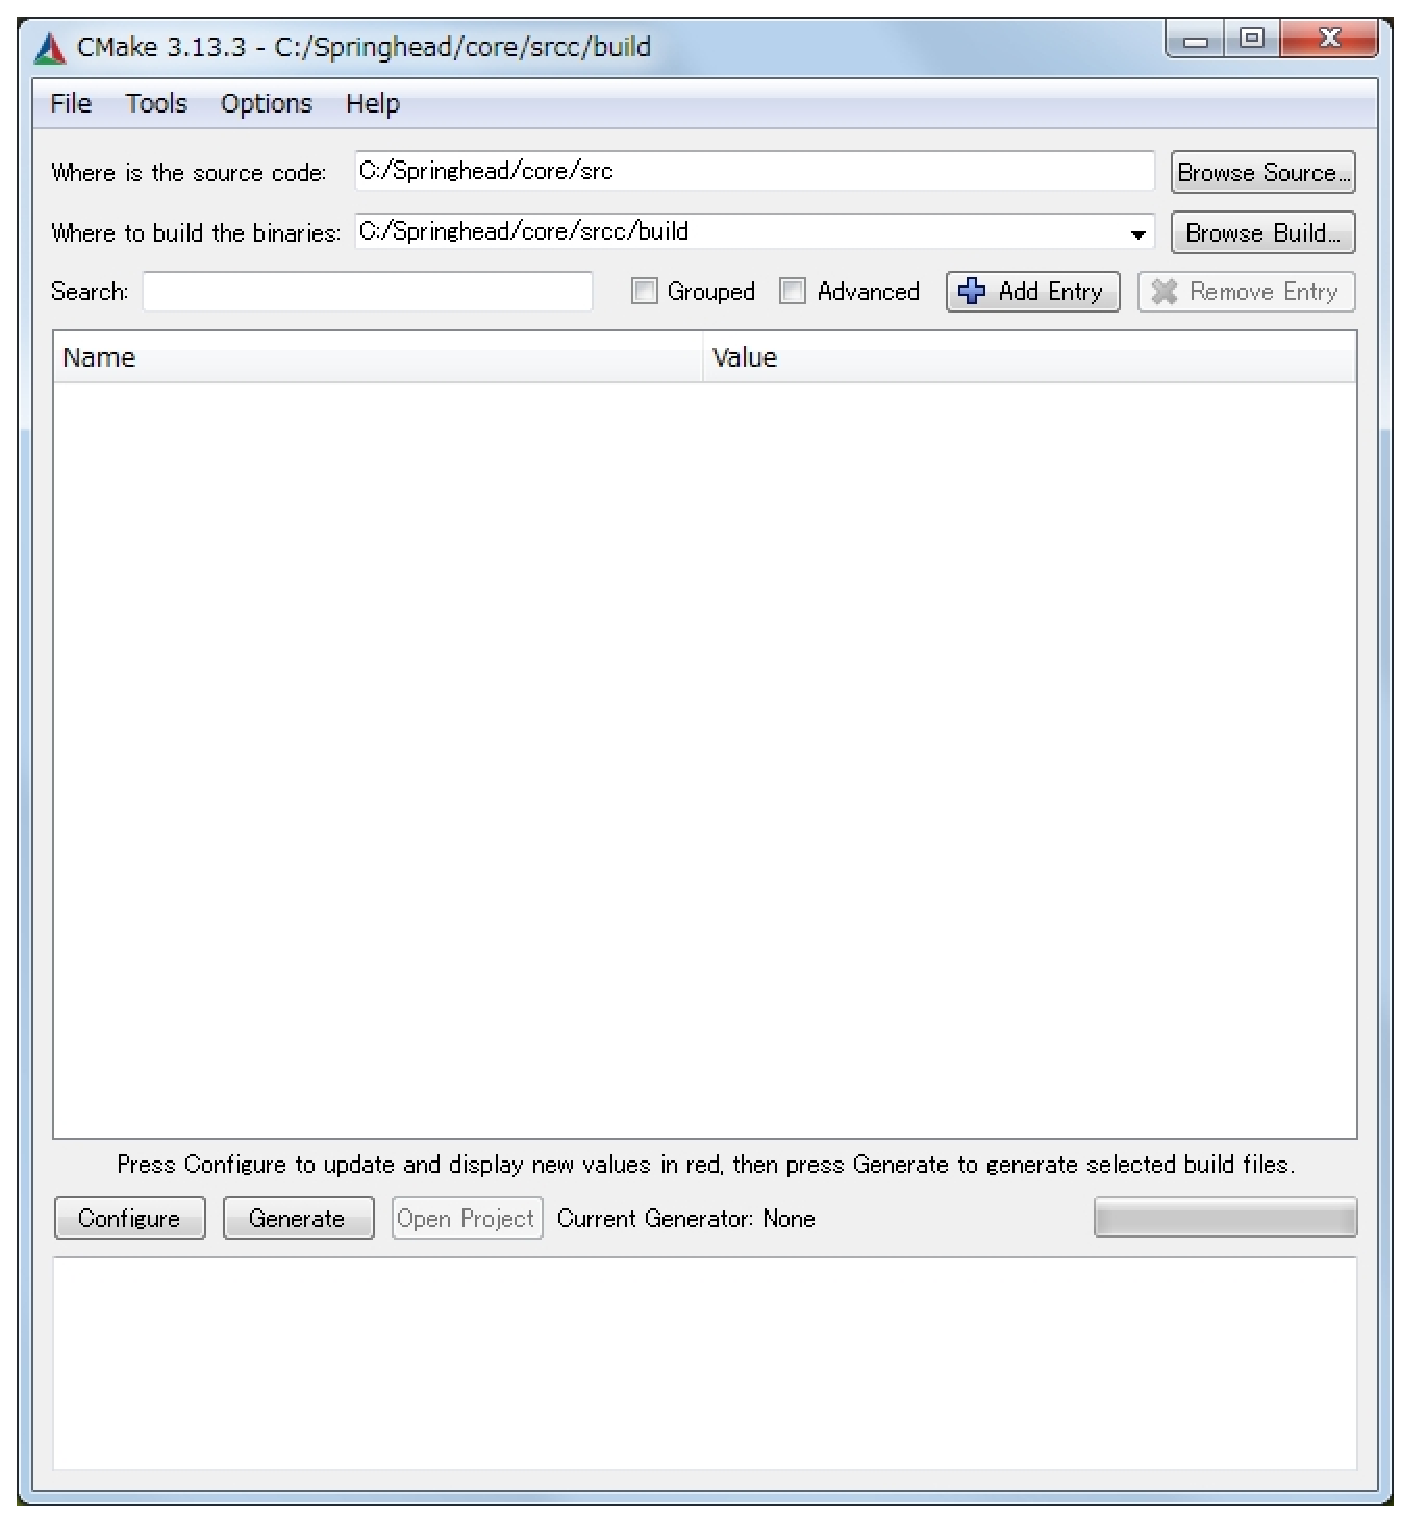
\includegraphics[width=0.35\textwidth]{fig/CmakeConfigure1.eps}
	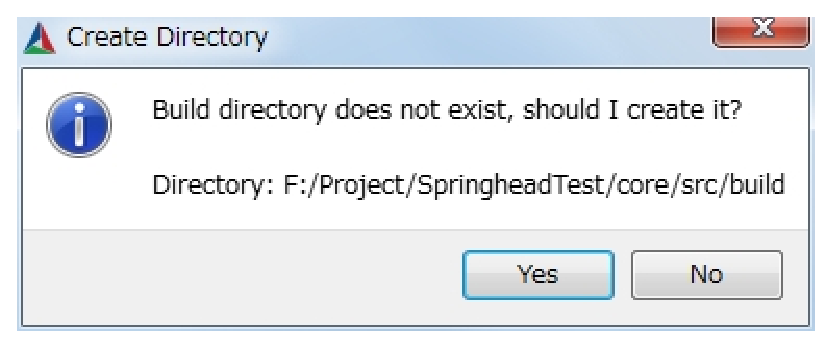
\includegraphics[width=0.2\textwidth]{fig/CmakeConfigure2.eps}
	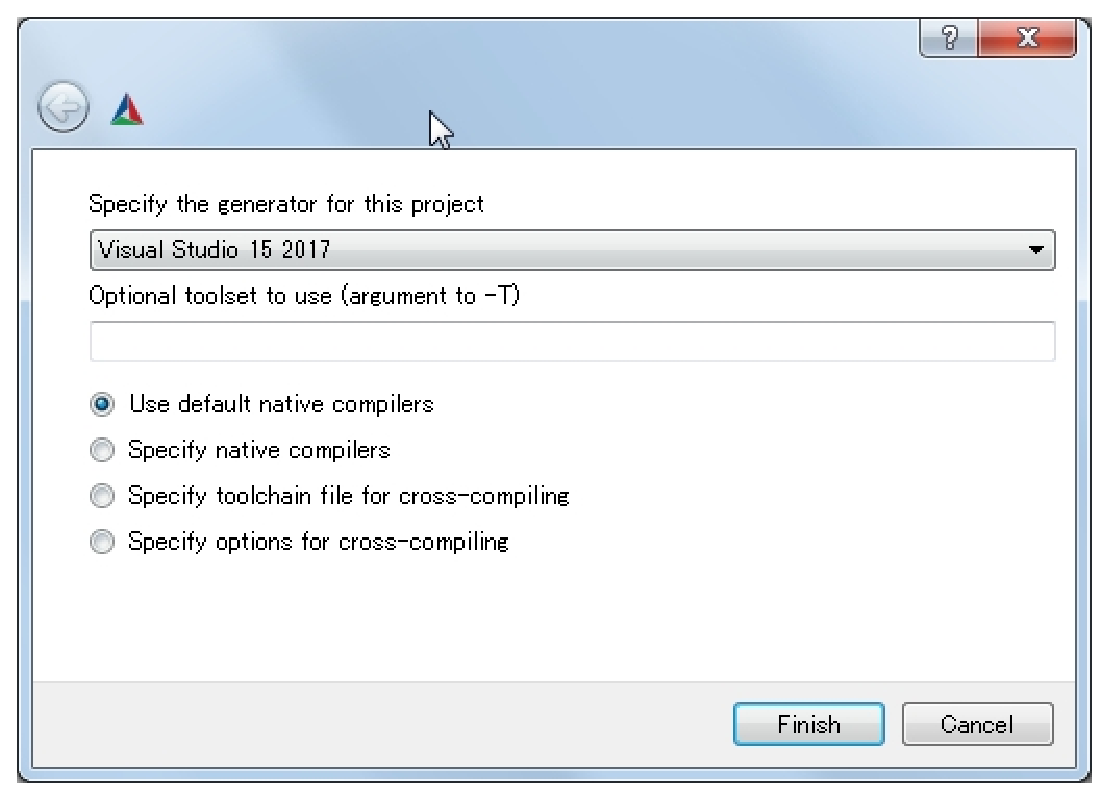
\includegraphics[width=0.3\textwidth]{fig/CmakeConfigure3.eps}
	\end{center}
	\caption{\cmake\ configure}
	\label{fig:CmakeConfigure}
	\end{figure}

	\Vskip{-.5\baselineskip}
	\build \KLUDGE ディレクトリがなければ作成するかどうか聞かれ(\KLUDGE 同中央図)\KLUDGE 、
	\KLUDGE 次にgenerator\KLUDGE 指定画面となります(\KLUDGE 同右図)\KLUDGE 。
	cmake version 3.15.0\KLUDGE では、
	generator\KLUDGE として図\ref{fig:CmakeGenerator}\KLUDGE のものが指定できます。

	\begin{figure}[h]
	\begin{center}
	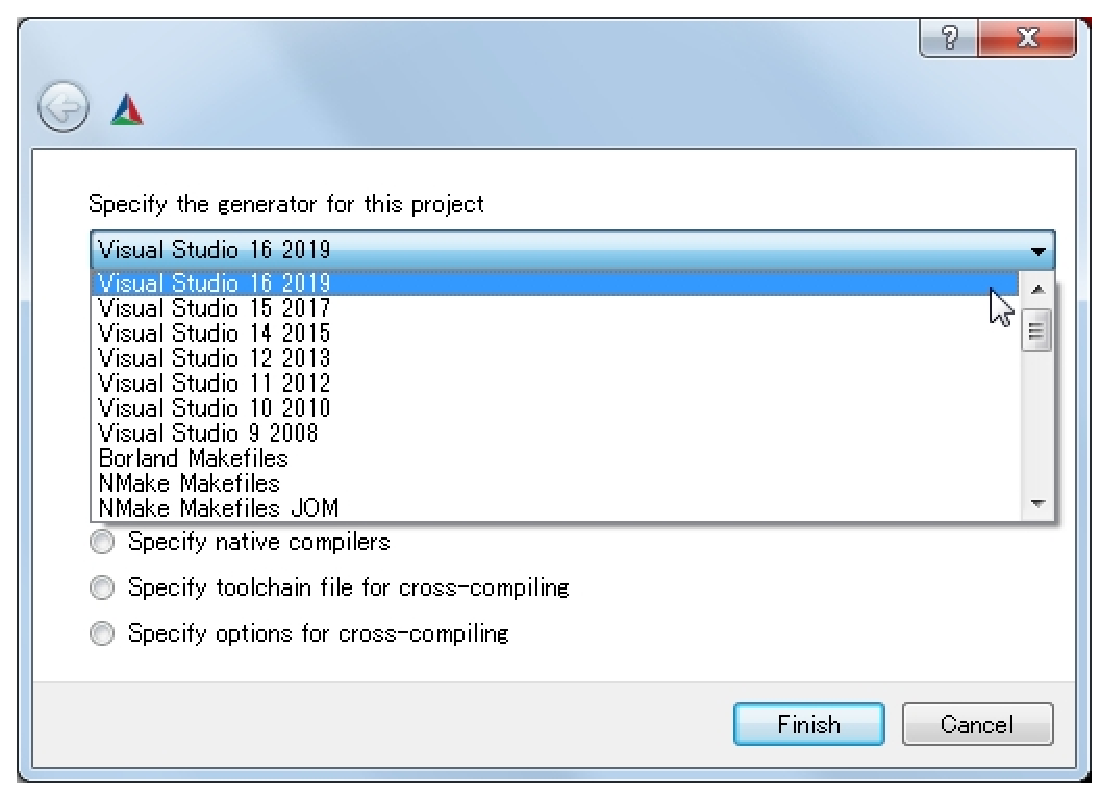
\includegraphics[width=0.3\textwidth]{fig/CmakeConfigure4.eps}
	\end{center}
	\caption{\cmake\ generator}
	\label{fig:CmakeGenerator}
	\end{figure}

	\KLUDGE 最後に図\ref{fig:CmakeConfigure} \KLUDGE 左図の下のGenerate\KLUDGE ボタンを押します。
\end{narrow}

\medskip
\noindent
\KLUDGE 以上で、\build \KLUDGE 以下にsolution/project file\KLUDGE などが生成されたはずです。

\bigskip

% end: 2.3.CmakeLibrary.tex
